\chapter{Propuesta}

En este trabajo se propone realizar la implementación en Dart de un sistema de inferencia de facetas de declasificación, que incluya el análisis de \textit{Type-based declassification}, mediante la realización de un plugin para entornos de desarrollo integrado (IDE). En este capítulo se detalla el problema de inferencia a resolver, las estrategias utilizadas para resolverlo y las restricciones de la solución.

\section{Problema de inferencia}
Para la formulación del problema, es posible asumir que la información de las facetas privadas de \textit{type-based declassification} se encuentra a disposición, debido a que algunos lenguajes de programación poseen herramientas para obtener dicha información.

\begin{defn}[Problema de inferencia]
  Dado un programa parcialmente tipado con facetas de declasificación, y completamente tipado con facetas privadas, encontrar la faceta de declasificación de las expresiones no tipadas, tal que se cumplan las reglas del sistema de tipos de type-based declassification.
\end{defn}

A continuación, se muestran algunos ejemplos de código parcialmente anotado con facetas de declasificación, con el objetivo de ilustrar la solución esperada al problema de inferencia.

\begin{ej} \ \\
  \label{ej1}
  \normalfont
\begin{lstlisting}
  bool login(String password, String guess) {
    return password.eq(guess);
  }
\end{lstlisting}
\end{ej}

En este caso, se quiere inferir que \texttt{password} tiene una faceta de declasificación que contiene al método \texttt{eq}, y que tanto el retorno de \texttt{login} como el parámetro \texttt{guess} dependen de la decisión que se tome sobre las facetas públicas por defecto que tendrán los métodos del \textit{core} del lenguaje.

\begin{ej} \ \\
  \normalfont
\begin{lstlisting}
  bool login(String<Top password, String guess) {
    return password.eq(guess);
  }
\end{lstlisting}
\end{ej}


Acá, se quiere inferir que el método \texttt{login} tiene a \texttt{Top} como faceta de declasificación, debido a la aplicación de la regla \texttt{TmH} de \textit{type-based declassification}.

\begin{ej} \ \\
  \normalfont
\begin{lstlisting}
  bool login(String password, String guess) {
    return password.hash().eq(guess);
  }
\end{lstlisting}
\end{ej}

En este caso ocurrió un encadenamiento de llamadas a métodos sobre \texttt{password}. La faceta de declasificación para \texttt{password} que resuelve el problema de inferencia contiene al método \texttt{hash}, al cual se le infiere una faceta de declasificación de retorno que contiene al método \texttt{eq}. Si se declara una faceta de declasificación de retorno para el método \texttt{eq}, entonces se infere esa misma faceta para el retorno del método \texttt{login}, por la aplicación de la regla \texttt{TmD} de \textit{type-based declassification}.

\begin{ej} \ \\
  \normalfont
\begin{lstlisting}
  void check(String<Bot s);

  bool<Top login(String<Top password, String guess) {
    check(password);
    return password.eq(guess);
  }
\end{lstlisting}
\end{ej}

En este caso, se debe reportar un error de flujo en el llamado a la función \texttt{check}, debido a que la faceta del argumento debe ser subtipo de la faceta del parámetro, esto es, \texttt{Top <: Bot} es una relación no válida.

\section{Gramática de tipos}
Como se vió en la sección \ref{schemes}, es necesario introducir variables de tipo para poder hacer inferencia. Además, se deben definir los otros tipos que serán utilizados internamente en el análisis.

\begin{defn}[Gramática de tipos]
  \normalfont
  $\tau := \alpha\ |\ \text{Obj}(\overline{l: \tau})\ |\ \tau \rightarrow \tau \ |\ \tau \vee \tau\ |\ \tau \wedge \tau \ |\ \text{Bot}\ |\ \text{Top}$
\end{defn}

Donde $\alpha$ es cualquier variable de tipo, $\text{Obj}(\overline{l: \tau})$ representa el tipo de un objeto, $l$ es un nombre de método, $\vee$ representa la operación \texttt{join} en la lattice, y $\wedge$ representa la operación \texttt{meet}.

\section{Consideraciones de diseño}

En el ejemplo \ref{ej1}, se mencionó sobre la decisión acerca de las facetas de declasificación de los métodos que pertenecen al \textit{core} de un lenguaje de programación. Para ilustrar la necesidad de esta decisión, veamos el siguiente ejemplo:

\begin{lstlisting}
  int<Bot getLength(String password) {
    return password.length
  }
\end{lstlisting}

Este método será aceptado o rechazado por las reglas del sistema de tipos, si la faceta de declasificación de retorno del campo \texttt{length} es \texttt{Bot} o \texttt{Top} respectivamente.

Si decidimos que la faceta de declasificación de retorno para métodos del \texttt{core} del lenguaje es \texttt{Top}, entonces cualquier operación que realicemos sobre el valor de retorno, retornará \texttt{Top}, lo cual es poco útil. Por lo tanto la decisión por defecto es que la faceta de declasificación de retorno para métodos del \textit{core} del lenguaje sea \texttt{Bot}.

Ahora, analicemos ambas posibilidades para la faceta de declasificación por defecto de los parámetros:

\begin{itemize}
  \item \texttt{Top} $\rightarrow$ \texttt{Bot}: Supongamos que el \textit{core} del lenguaje posee un método \texttt{identity}, que dado un \texttt{x}, retorna \texttt{x}. Si tomamos esta decisión, entonces el método \texttt{identity} podrá ser usado como declasificador universal, como por ejemplo \texttt{identity(password)}.
  \item \texttt{Bot} $\rightarrow$ \texttt{Bot}: Esta elección restringe las facetas de declasificación de los argumentos utilizados a \texttt{Bot}, lo cual también podría ser considerado poco útil. Sin embargo, al retornar un valor con faceta de declasificación \texttt{Bot}, cualquier operación podrá ser utilizada sobre ese valor.
\end{itemize}

Haciendo un balance, se considera que la opción \texttt{Bot} $\rightarrow$ \texttt{Bot} tiene el mejor equilibrio entre utilidad y seguridad, por lo que es la opción por defecto considerada. Sin embargo, es deseable que la herramienta se pueda configurar para elegir otra alternativa.

\section{Generación de constraints de subtyping}
Como se mencionó en la sección \ref{constraints}, el uso de constraints permite presentar un algoritmo de inferencia como una fase de generación de constraints, y una fase de resolución de constraints. A continuación se muestran ejemplos de la generación de constraints para distintas expresiones, y luego un algoritmo en pseudo-lenguaje. De ahora en adelante, se usará el término \textit{faceta} para referirse a las facetas de declasificación.

\begin{ej}\ \\
  \normalfont
  \label{gen1}
\begin{lstlisting}[mathescape=true]
  bool<$\alpha$ check(String<Top password, String<$\beta$ guess) {
    return password == guess; /* $\gamma$ */
  }
\end{lstlisting}

\begin{enumerate}
  \item $\gamma <: \alpha$
  \item $\beta <: \text{Bot}$
  \item $\text{Top} <: \text{Obj}(\text{==: }\text{Bot} \rightarrow \text{Bot}), \gamma$
\end{enumerate}
\end{ej}

En este ejemplo, la constraint 1 se genera por la regla que indica que la faceta de la expresión de retorno del método ($\gamma$) debe ser subtipo de la faceta de retorno del método ($\alpha$). La constraint 2 se genera por la regla que indica que la faceta del argumento en una llamada a método ($\beta$), debe ser subtipo de la faceta del parámetro correspondiente de ese método ($\text{Bot}$, ya que el método \texttt{==} es parte del \textit{core} del lenguaje).

La constraint 3 se genera por la llamada al método \texttt{==}, indicando que la faceta del objetivo de la llamada (\texttt{Top}) debe ser subtipo de un objeto que contenga al método. Las constraints que se generan por llamadas a métodos, poseen además la faceta que corresponde a la expresión de esa llamada ($\gamma$), debido a la posible aplicación de la regla \texttt{TmH} en caso de que la relación de subtyping no sea válida. En este caso, la relación no es válida pues \texttt{Top} no es subtipo de $\text{Obj}(\text{==: }\text{Bot} \rightarrow \text{Bot})$.

\begin{ej}\ \\
  \normalfont
  \label{gen2}
\begin{lstlisting}[mathescape=true]
  class Person {
    bool<Top permission => true;
  }

  class Foo {
    String<$\alpha$ foo(Person<$\beta$ p) {
      String<Bot ret = "denied";
      if (p.permission /* $\gamma$ */) ret = "exito";
      return ret;
    }
  }
\end{lstlisting}

\begin{enumerate}
  \item $\text{Bot} <: \text{Top}$
  \item $\text{Bot} <: \text{Bot}$
  \item $\beta <:\text{Obj}(\text{permission: }\text{Top}), \gamma$
  \item $\text{Bot} <: \text{Bot}$
  \item $\text{Top} <: \text{Bot}$
  \item $\text{Bot} <: \alpha$
\end{enumerate}
\end{ej}

En este ejemplo, la constraint 1 se genera por la relación entre la expresión de retorno y la faceta de retorno del método \texttt{permission}. Notar que el literal \texttt{true} tiene una faceta por defecto \texttt{Bot}. La constraint 2 se genera por la relación entre los lados izquierdo y derecho de la asignación a la variable \texttt{ret}. La constraint 3 se genera por la llamada al método \texttt{permission} sobre el parámetro \texttt{p}. Las constraints 4 y 5 se generan por la asignación a la variable \texttt{ret} en el cuerpo del condicional. La primera, expresa la relación entre el lado derecho de la asignación y el lado izquierdo, y la segunda expresa la relación entre el PC y el lado izquierdo de la asignación. La constraint 6 se genera por la relación entre la expresión de retorno del método y el retorno del método.

\begin{ej}\ \\
  \normalfont
  \label{gen3}
\begin{lstlisting}[mathescape=true]
  int<$\alpha$ calc(num<$\beta$ n) {
    int<$\text{Top}$ ret = 1 + n.ceil() /* $\gamma$ */;
    ret = ret + n.floor() /* $\delta$ */;
    return ret;
  }
\end{lstlisting}

\begin{enumerate}
  \item $\text{Bot} <: \text{Top}$
  \item $\beta <: \text{Obj}(\text{ceil}: [\ ] \rightarrow \text{Bot}),\ \gamma$
  \item $\text{Top} <: \text{Top}$
  \item $\beta <: \text{Obj}(\text{floor}: [\ ] \rightarrow \text{Bot}),\ \delta$
  \item $\text{Top} <: \alpha$
\end{enumerate}
\end{ej}

En este ejemplo, las constraints 1 y 3 se generan por la asignación a la variable \texttt{ret}. En cambio, las constraints 2 y 4 se generan por la llamada a los métodos \texttt{ceil} y \texttt{floor} del parámetro \texttt{n}. Este ejemplo es útil para mostrar el uso de la operación \texttt{meet} en el paso de resolución de constraints, debido a que la faceta de la variable $\beta$ se debe resolver considerando la intersección entre dos facetas.

% TODO arreglar esa ref
En la figura 3.1 se muestra el algoritmo para la generación de constraints de un nodo determinado del árbol de sintaxis abstracta.

\begin{figure}[ht]
  \centering
  \label{pseudogen}
  \begin{mdframed}
    \begin{algorithmic}
      \Function{Constraint\_Generator}{node, pc}
          \State $\text{cs}\gets \{\}$
          \If {node is MethodInvocation}
            \State cs.insert(methodTarget <: Obj(methodName: methodSignature), callExpression)
            \State cs.insert(callExpression <: methodReturn)
            \For {argument$\gets$ methodArgument}
              \State cs.insert(argument <: correspondingParameter)
            \EndFor
          \ElsIf {node is ReturnStatement}
            \State cs.insert(returnExpression <: methodReturn)
            \State cs.insert(pc <: methodReturn)
          \ElsIf {node is AssignmentExpression}
            \State cs.insert(rightHand <: LeftHand)
            \State cs.insert(pc <: LeftHand)
          \ElsIf {node is IfExpression}
            \State $\text{pc}\gets \text{conditionExpression}$
          \EndIf
          \State \Return cs,pc
      \EndFunction
    \end{algorithmic}
  \end{mdframed}
  \caption{Algoritmo de generación de constraints}
\end{figure}


\section{Resolución de constraints}

El siguiente paso del algoritmo de inferencia es la resolución de un set de constraints.

\subsection{Simplificación y eliminación de constraints}
El primer paso del algoritmo de resolución de constraints es la eliminación de constraints \textit{obvias}. Esto es, la eliminación de las constraints \texttt{Bot <: X} y \texttt{X <: Top}. Así, en el ejemplo \ref{gen2}, las constraints resultantes son:

\begin{enumerate}
  \item $\beta <:\text{Obj}(\text{permission: }\text{Top}), \gamma$
  \item $\text{Top} <: \text{Bot}$
\end{enumerate}

Y para el ejemplo \ref{gen3}:

\begin{enumerate}
  \item $\beta <: \text{Obj}(\text{ceil}: [\ ] \rightarrow \text{Bot}),\ \gamma$
  \item $\beta <: \text{Obj}(\text{floor}: [\ ] \rightarrow \text{Bot}),\ \delta$
  \item $\text{Top} <: \alpha$
\end{enumerate}
\subsection{Agrupación de constraints}
El siguiente paso es agrupar las constraints sobre la misma variable de tipo, usando las siguientes reglas:

\begin{itemize}
  \item \texttt{x <: y}, \texttt{x <: z} $\rightarrow$ \texttt{x <: y }$\wedge$\texttt{ z}
  \item \texttt{y <: x}, \texttt{z <: x} $\rightarrow$ \texttt{y }$\vee$\texttt{ z <: x}
\end{itemize}

Así, el ejemplo \ref{gen3} simplificado, se reduce a dos constraints:

\begin{enumerate}
  \item $\beta <: \text{Obj}(\text{ceil}: [\ ] \rightarrow \text{Bot})\ \wedge\ \text{Obj}(\text{floor}: [\ ] \rightarrow \text{Bot})$
  \item $\text{Top} <: \alpha$
\end{enumerate}


\subsection{Unificación}
En este paso, se materializan las operaciones \texttt{meet} y \texttt{join}, se comprueba la validez de las constraints y se realizan substituciones, de forma iterativa.

\subsubsection{Meet y Join}
Cuando se tiene un tipo $x \wedge y$ o $x \vee y$, donde $x$ e $y$ no tienen variables de tipo, entonces se puede materializar la operación sobre la lattice correspondiente.

\begin{figure}[ht]
  \centering
  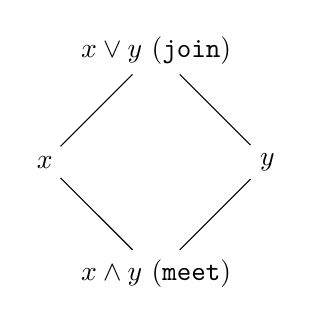
\begin{tikzpicture}[node distance=2cm]
    \node(Top) 												{$x \vee y$ (\texttt{join})};
    \node(y)		[below right of=Top]			{$y$};
    \node(x)					[below left of=Top] 			{$x$};
    \node(Bot)  [below right of=x] {$x \wedge y$ (\texttt{meet})};
    \draw(Top)      -- (y);
    \draw(Top)      -- (x);
    \draw(x)      -- (Bot);
    \draw(y)      -- (Bot);
  \end{tikzpicture}
  \label{latticexy}
  \caption{Operaciones sobre lattice}
\end{figure}

En el ejemplo \ref{gen3} reducido, se materializa la operación \texttt{meet} del lado derecho de la constraint 1, por lo que las constraints quedan como sigue:

\begin{enumerate}
  \item $\beta <: \text{Obj}(\text{ceil}: [\ ] \rightarrow \text{Bot},\ \text{floor}: [\ ] \rightarrow \text{Bot})$
  \item $\text{Top} <: \alpha$
\end{enumerate}

\subsubsection{Comprobación de constraints}
Cuando una constraint representa una relación no válida, existen dos posibilidades:

\begin{enumerate}
  \item Si la constraint no proviene de una invocación a método, se debe reportar un error.
  \item En caso contrario, se debe reemplazar, en el set de constraints, toda aparición de la faceta de expresión de la constraint, por \texttt{Top}. En este caso no se debe reportar error.
\end{enumerate}

En el ejemplo \ref{gen1}, la constraint 3 proviene de invocación a método y representa una relación de subtyping no válida. Luego, se debe reemplazar la variable de tipo $\gamma$ por \texttt{Top}:

\begin{enumerate}
  \item $\text{Top} <: \alpha$
  \item $\beta <: \text{Bot}$
  \item $\text{Top} <: \text{Obj}(\text{==: }\text{Bot} \rightarrow \text{Bot}), \gamma$
\end{enumerate}

En cambio, en el ejemplo \ref{gen2} simplificado, la constraint \texttt{Top <: Bot} representa una relación no válida que no proviene de invocación a método, por lo que un error debe ser reportado.

\subsubsection{Substitución}
